%========================================
\chapter{Requirement Specification \& Methodology}
%========================================

\section{Software Development Life Cycle (SDLC) Model}

AgriQueue adopted an Agile Iterative methodology tailored for rapid multi-tier development, iterative machine learning model tuning, and continuous stakeholder feedback:

\begin{figure}[H]
\centering
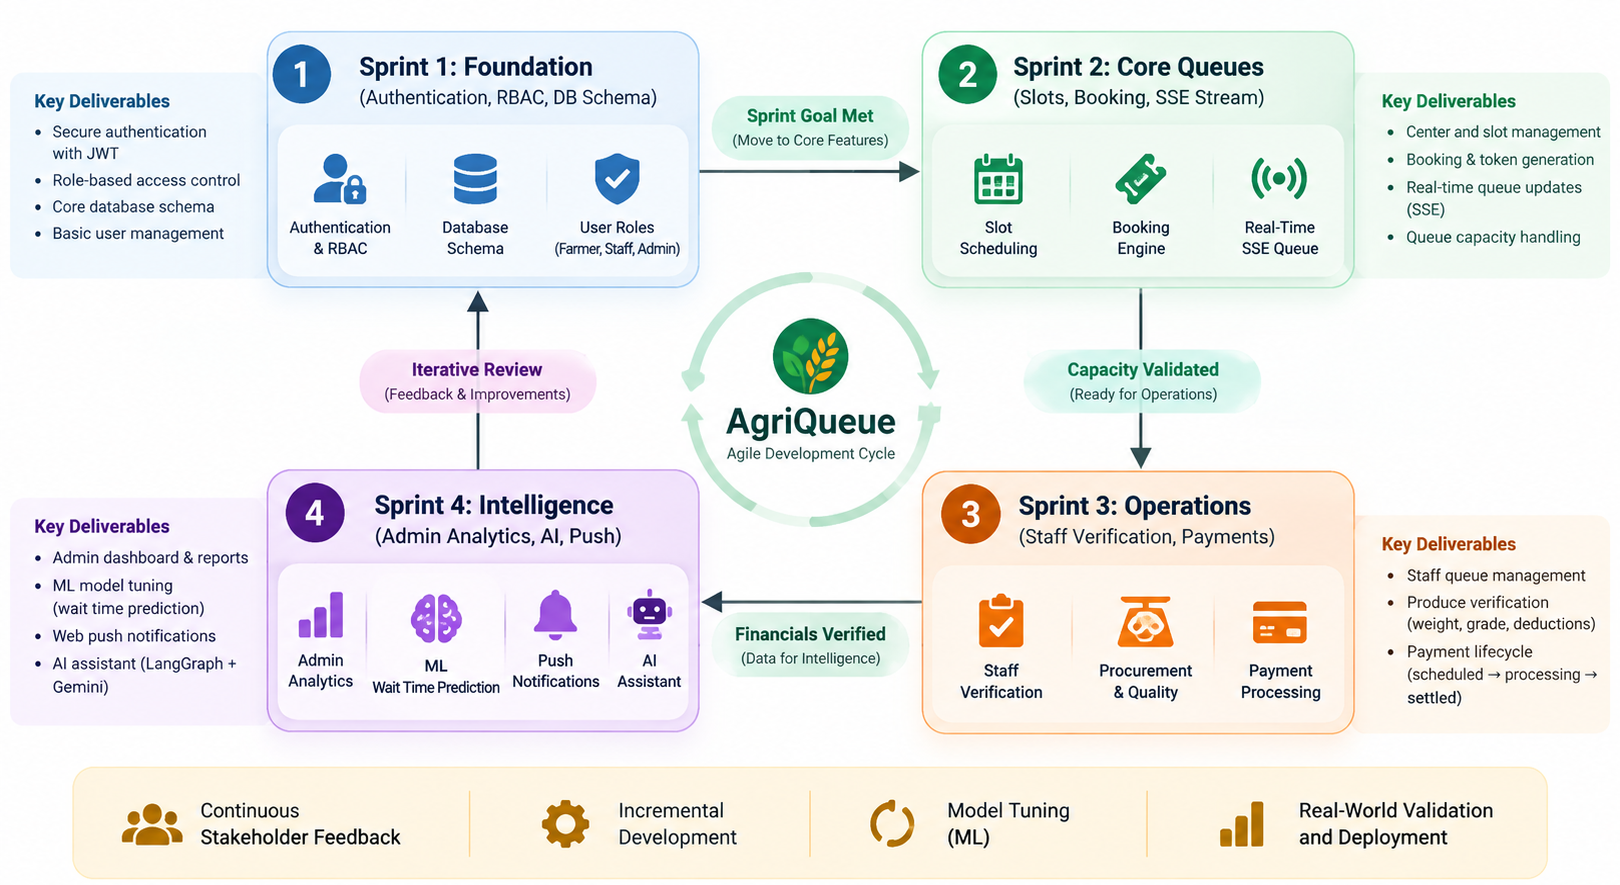
\includegraphics[width=\textwidth]{img/sdlc_agile_lifecycle.png}
\caption{Agile Iterative Sprint Lifecycle for AgriQueue}
\label{fig:sdlc}
\end{figure}

\begin{itemize}
  \item \textbf{Sprint 1 (01--06 Sep 2026):} Domain modeling, database migrations, JWT authentication, and center/crop configuration.
  \item \textbf{Sprint 2 (07--12 Sep 2026):} Slot capacity logic, booking engine, token assignment, and live queue SSE streaming.
  \item \textbf{Sprint 3 (13--18 Sep 2026):} Staff operational workflow, weighment deductions, automated net calculation, and payment lifecycle.
  \item \textbf{Sprint 4 (19--25 Sep 2026):} HistGBR model training, LangGraph AI command agent, WebPush alerts, and cloud deployment.
\end{itemize}

\section{System Use Cases}

The platform supports distinct actor interactions across the three operational roles:

\begin{figure}[H]
\centering
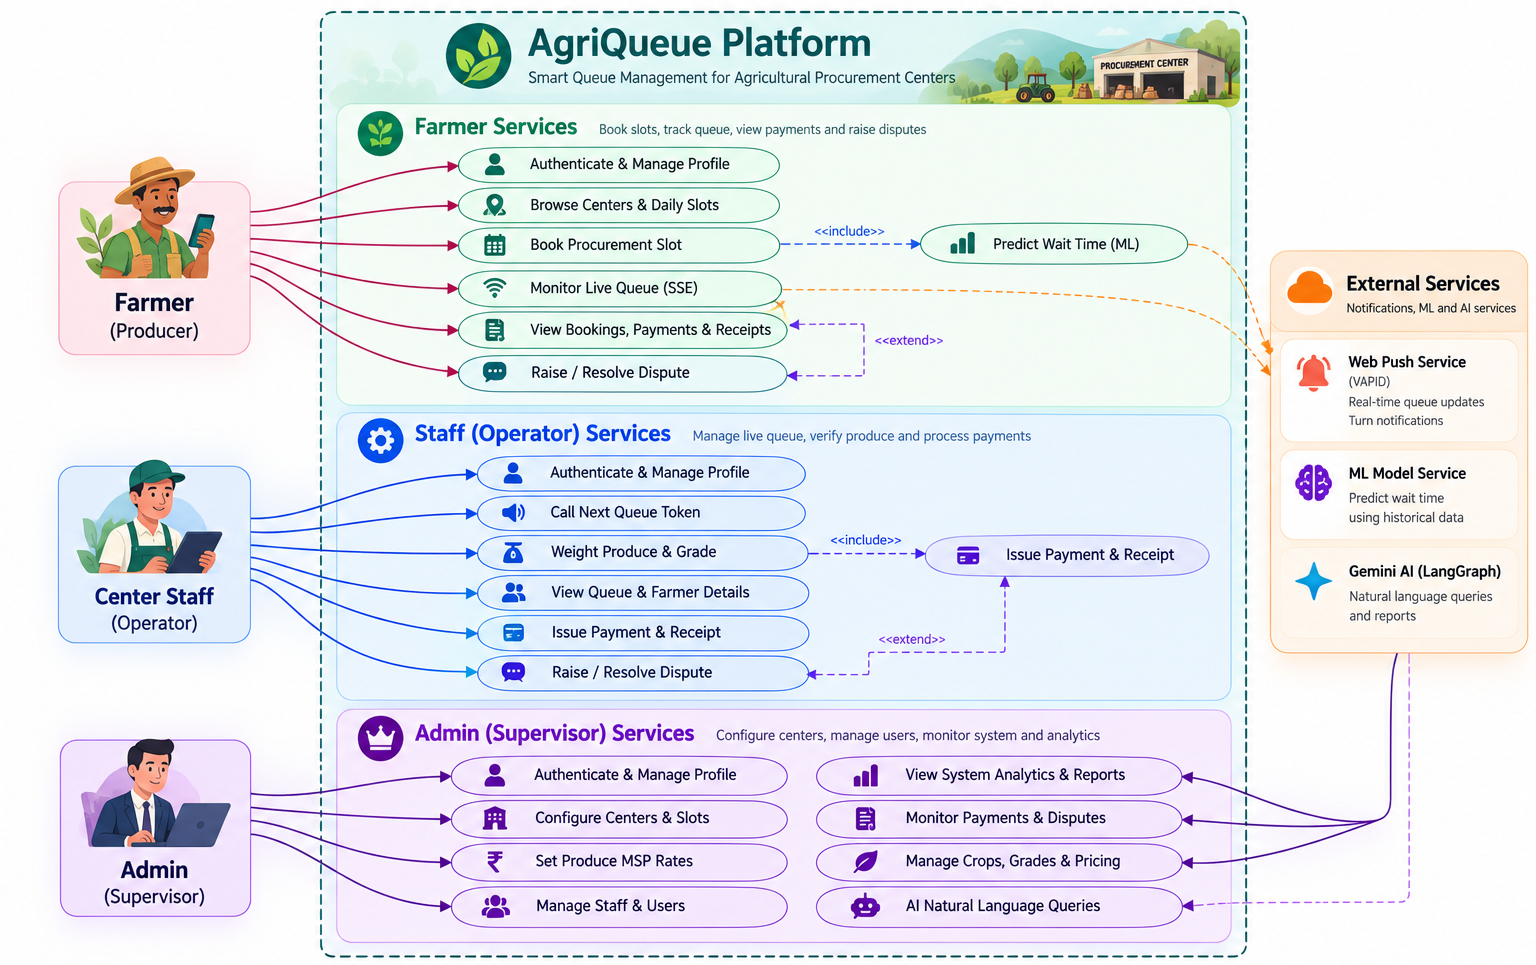
\includegraphics[width=\textwidth]{img/usecase_clean.png}
\caption{Comprehensive UML Use Case Diagram for AgriQueue Actors and System Boundary}
\label{fig:usecase}
\end{figure}

\section{Functional Requirements}

\subsection{Farmer Module}
\begin{itemize}
  \item Self-registration with validated mobile number, full name, district, and village.
  \item Secure login with HTTP-only cookie-based authentication.
  \item Real-time discovery of nearby procurement centers and operational crop types.
  \item Inspection of daily time slots with visual availability indicators (Available, Full, Expired).
  \item Slot reservation with dynamic capacity validation and ML-estimated wait calculation.
  \item Live token tracking via low-latency Server-Sent Events with countdown metrics.
  \item Inspection of procurement receipts and tracking payment settlement states.
  \item Browser push notification subscription for queue summons and disbursement alerts.
\end{itemize}

\subsection{Staff Module}
\begin{itemize}
  \item Role-authenticated login restricted to designated procurement center locations.
  \item Real-time dashboard of daily registered arrivals sorted by sequential token numbers.
  \item Immediate status mutation to \textit{Serving} with synchronized client-side notification.
  \item Digital entry of gross vehicle weight, tare weight, tare deductions, and moisture percentage.
  \item Automated evaluation of net payable amount using government MSP lookup tables.
  \item Initiation and status management of digital payment transactions (Scheduled $\to$ Settled).
\end{itemize}

\subsection{Admin Module}
\begin{itemize}
  \item System-wide operational dashboard visualizing total centers, bookings, and financial turnover.
  \item Administrative CRUD controls for centers, operating hours, capacity quotas, and crop MSP rates.
  \item Staff profile provisioning and center assignment management.
  \item Audit trail logging and administrative review of user dispute tickets.
\end{itemize}

\section{Non-Functional Requirements}

\begin{table}[H]
\centering
\caption{AgriQueue Non-Functional Requirements Matrix}
\label{tab:nfr}
\renewcommand{\arraystretch}{1.2}
\begin{tabular}{|p{3cm}|p{10.5cm}|}
\hline
\textbf{Category} & \textbf{Specification and Threshold} \\ \hline
Performance & 95\% of REST API responses served in under 500 milliseconds \\ \hline
Real-Time Delivery & Queue mutations broadcast via SSE to connected clients within 5 seconds \\ \hline
Concurrency & Architectural support for 1,000+ simultaneous active farmer sessions \\ \hline
Security & Argon2id password hashing, HTTP-only JWT storage, and CORS whitelisting \\ \hline
ML Precision & Wait-time prediction error within $\pm$10 minutes ($R^2 \geq 0.95$) \\ \hline
Availability & 99.5\% system uptime maintained throughout operational hours (8 AM -- 6 PM) \\ \hline
\end{tabular}
\end{table}

\section{System Interfaces}

\subsection{Software Interfaces}
\begin{itemize}
  \item \textbf{User Interface:} React 19 single-page application utilizing Lucide icons and modern CSS.
  \item \textbf{Application Framework:} FastAPI ASGI web framework running under Uvicorn.
  \item \textbf{Relational Database:} PostgreSQL 15 accessed asynchronously through SQLAlchemy 2.0 and \texttt{asyncpg}.
  \item \textbf{Inference Engine:} scikit-learn HistGradientBoosting regression pipeline serialized via Joblib.
  \item \textbf{Generative Agent:} LangChain and LangGraph orchestration over Google Gemini Flash APIs.
  \item \textbf{Push Protocols:} WebPush VAPID protocol managed through \texttt{pywebpush}.
\end{itemize}

\subsection{Communication Interfaces}
\begin{itemize}
  \item \textbf{HTTPS REST API:} Standardized JSON payloads over TLS 1.3 encryption.
  \item \textbf{Server-Sent Events (SSE):} Persistent HTTP text/event-stream connection for unidimensional push.
  \item \textbf{Browser WebPush:} Secure VAPID-authenticated event delivery across disparate networks.
\end{itemize}

\section{Hardware and Operating Specifications}

\begin{table}[H]
\centering
\caption{System Hardware Requirements}
\label{tab:hw}
\renewcommand{\arraystretch}{1.2}
\begin{tabular}{|p{3.2cm}|p{5.0cm}|p{5.0cm}|}
\hline
\textbf{Resource} & \textbf{Minimum Specification} & \textbf{Recommended Production} \\ \hline
Server CPU & 2 Cores (x86-64 / ARM64) & 4+ Cores (2.5+ GHz) \\ \hline
Server RAM & 4 GB & 8--16 GB High-Speed DDR4 \\ \hline
Disk Storage & 20 GB NVMe SSD & 100+ GB Managed Cloud Storage \\ \hline
Network & 10 Mbps Dedicated Uplink & 100+ Mbps Redundant Connection \\ \hline
Client Device & Modern Smartphone / PC & 4G/5G Connectivity, 2+ GB RAM \\ \hline
\end{tabular}
\end{table}

\section{General Constraints}
\begin{itemize}
  \item \textbf{Network Connectivity:} Active internet connection required; offline synchronization not supported in initial release.
  \item \textbf{Browser Compatibility:} Web Push features require modern standards-compliant browsers (Google Chrome, Mozilla Firefox, Microsoft Edge).
  \item \textbf{Hardware Instrumentation:} Weighbridge readings are entered manually by verified center staff rather than via IoT telemetry.
  \item \textbf{Localization:} User interface localization currently provided in English, with multi-language regional support scheduled for Phase II.
\end{itemize}
